\documentclass[10pt,twocolumn]{article}

\usepackage[margin=0.75in]{geometry}
\usepackage[T1]{fontenc}
\usepackage[utf8]{inputenc}
\usepackage{times}
\usepackage{microtype}
\usepackage{amsmath,amssymb}
\usepackage{booktabs}
\usepackage{graphicx}
\usepackage{subcaption}
\usepackage{tabularx}
\usepackage{enumitem}
\usepackage{hyperref}
\usepackage{tikz}
\usepackage{verbatim}
\usepackage{fancyvrb}
\usepackage[review]{acl} 
\usetikzlibrary{arrows.meta,calc,positioning}

\setlength{\textfloatsep}{8pt plus 2pt minus 2pt}
\setlength{\floatsep}{8pt plus 2pt minus 2pt}
\setlength{\intextsep}{8pt plus 2pt minus 2pt}
\setlength{\abovecaptionskip}{4pt}
\setlength{\belowcaptionskip}{-2pt}
\setlist[itemize]{leftmargin=*, topsep=2pt, itemsep=1pt, parsep=0pt}

\title{\textbf{Belief--Action Gaps in Language-Model Agents}}
\author{
Anonymous
}
\date{}

\begin{document}
\maketitle

% ===== Collaboration notes for the 4-page EMNLP draft =====
% [Behavioral owner] Own the integrated literature paragraph, the descriptive
% evidence section, Table 1, and the failure-state behavioral figure.
% [White-box owner] Keep your contribution to short inline result sentences; do
% not add a separate white-box table.
% [IRL owner] Keep your contribution to one short estimator paragraph and at
% most one compressed validation sentence.
% [Reasoning owner] Section 4 should prioritize patching/steering. Keep the
% auxiliary revealed-CoT diagnostic only if space remains after the causal result.

\begin{abstract}
Language-model (LM) agents may fail because they lack task-relevant state information, pursue an objective misaligned with the user's intent, or fail to convert represented information into action. In this work, we study the third case through the \emph{belief--action gap}: the expected regret of the agent's chosen action under a probe-estimated belief distribution and a learned state value function. In text-rendered gridworlds, we measure state knowledge using both behavioral and representation-level probes, and estimate objective-consistent action values using one-step inverse reinforcement learning (IRL) over exact next states. We find that the model's representations encode task-relevant state and value structure more reliably than its chosen actions. Optimal-action supervised IRL recovers near-perfect action preferences, while agent-action supervision is much weaker, and behavioral probes reveal cases where the model reports local obstacles correctly yet still acts against them. We then test whether this gap is causal by intervening on trajectory representations with patching and steering both pre- and post- reasonin. The interventions show that decoded state information does not always control the final action: actions follow patched reasoning traces, but changing pre-reasoning activations alone does not reliably change the output. This suggests that a gap arises when state information is present but not used in choosing the action. This gives a causal diagnostic framework for agents that know relevant state information but fail to act on it.
\end{abstract}

\section{Introduction}
In order to engineer reliable, safe, and trustworthy language model (LM) agents, it is essential to understand not only the actions taken by agents but also how agents arrive at them. In sequential settings, a chosen action depends on at least three components: the agent's belief about the current state, the objective or action-value structure it is effectively optimizing, and the reasoning pathway that converts beliefs and values into a committed action. Failures can therefore arise because task-relevant state information is absent, because the inferred objective is misaligned with the user's intent, or because represented information is not used to select the final action. We study the third case through the \emph{belief--action gap}: the excess expected cost of the taken action relative to the best action under the agent's inferred beliefs and action values.

This distinction is not merely theoretical -- it is of practical import for the interpretability and safety of LM agents. 
An undesirable action taken by an agent can reflect different, potentially overlapping, internal failure modes. For interpretability, state-estimation failure, objective misspecification, and action-selection failure require different
explanations and interventions. For safety, action-level evaluation alone cannot reveal whether failures come from missing information, unused information, or a conflicting objective. This ambiguity is central to analyses of deceptive alignment, alignment faking, and sandbagging
\cite{hubinger2019risks,greenblatt2024faking,vanderweij2025sandbagging}.

Many existing methods address these components separately. Maximum-entropy inverse reinforcement learning and later work on goal-directedness and utility estimation provide tools for inferring objectives or action values from behavior \cite{ziebartMaximumEntropyInverse2008a,macdermott_measuring_2024,mazeika_utility_2025,bellot2025limits}. Representational probes recover structured state information from hidden activations, and behavioral probes provide a complementary estimate of what the model can explicitly report about the current state \cite{alain2016understanding,li2023emergent,nanda-etal-2023-emergent,gurnee2024language,arghal2026behavioural,martorell_text_2026}. Intervention-based interpretability asks whether such information is causally implicated rather than merely decodable: causal tracing and model editing localize factual computations \cite{meng2022locating}, activation patching supports causal localization of model behavior \cite{kramar2024atpstar}, representation steering manipulates high-level properties \cite{zou2023representation}, and chain-of-thought faithfulness studies show that exposed reasoning can diverge from the computation that determines the answer \cite{lanham2023measuring}. Yet these tools are rarely combined to ask whether an LM agent that encodes state information and supports objective-consistent preferences actually uses that information to choose its own action.

We operationalize this decomposition in text-rendered gridworlds, \textit{DoorKeyEnv}, using representational probes, behavioral probes, one-step inverse reinforcement learning over exact next states, and reasoning-trace interventions.
We find that LM agents can encode task-relevant state information and
objective-consistent action structure without reliably using them to choose their own actions: representational probes and behavioral probes recover relevant state information, one-step IRL recovers near-perfect optimal-action preferences more reliably than the model's realized actions. %We then show that \textcolor{red}{[summarize results of intervention analyses]}. %[add a sentence or two on the contribution or significance of these results.]}% and intervention analyses test whether this information affects behavior only when it lies on the active reasoning pathway for the action. % [headline causal result ]

Our contributions are four descriptive answers to the belief--action-gap. (1) We ask whether state beliefs are decodable from activations, and
show that pre-reasoning representations encode strong task-relevant state information. (2) We ask whether those activations support a coherent action-value structure, and show that one-step IRL recovers near-perfect optimal-action preferences more reliably than the model's realized actions. (3) We ask whether reasoning reduces the gap and at what cost to belief precision, and show that post-reasoning actions are better aligned with the learned value structure even as state beliefs become more diffuse. (4) We ask whether failure states exhibit correct local reports alongside inconsistent actions, and show that behavioral probes can recover the relevant local wall
facts even when the agent still acts against them. Section~4 then extends these descriptive diagnostics with reasoning-trace interventions.

% % [IRL owner: insert one headline empirical result clause here if space allows.]
% We then combine these measurements to identify failure states where accurate wall judgments coexist with inconsistent actions, and we study whether reasoning is causally implicated using chain-of-thought-related interventions on matched and failure-focused slices.
% % [Intervention owner: insert one headline causal result clause here if space allows.]
% Sections 2--5 define the belief estimators, the action-value estimator, the behavioral gap diagnostics, and the reasoning-trajectory analysis.

\section{Estimating Beliefs and Values}
We study a text-rendered gridworld, \textit{DoorKeyEnv}, in which an LM agent must navigate to a goal while tracking its position and collect a key to open a locked door blocking its path \cite{arghal2026behavioural}.
Appendix~\ref{app:environment} gives a summary
of the environment, state variables, and action space used for the probes and value estimator.

\paragraph{Representational belief.}
Representational belief is decoded from pre-reasoning activations. In \textit{DoorKeyEnv}, the state is $s_t=(x_t,y_t,\texttt{has\_key}_t,\texttt{door\_open}_t)$. Linear probes estimate task-relevant state variables from the activation vector at the last input token before chain-of-thought generation.

\paragraph{Behavioral belief.}
Behavioral belief is elicited with single-step, history-free prompts built from the current rendered grid. We use directional wall probes, object-direction probes for the key, door, and goal, and action-conditioned probes for immediate move consequences. Readouts include greedy sampling at $\text{temperature}=0.0$, repeated sampling at $\text{temperature}=0.7$, exposed logprob diagnostics, and Monte Carlo-sampled answers. We also compute a \emph{local contradiction rate}, where the chosen action matches a direction that the model judged blocked, and an \emph{A$^*$-conditioned gap rate}, where the action is non-optimal despite a correct wall judgment.

% [IRL OWNER] Keep this paragraph short. Add at most one headline empirical sentence
% after it. Do not introduce alternate IRL variants or extra tables.
\paragraph{Action value.}
We use one-step IRL as the operational estimator of action value \cite{ng2000algorithms, ziebartMaximumEntropyInverse2008a}. For state $s$ and action $a$, let $T(s,a)$ be the exact next state. We learn a state value $g_\theta$ and induce a Boltzmann policy \cite{ziebartMaximumEntropyInverse2008a, skalse_misspecification_2023};
\[
p_\theta(a \mid s) \propto \exp\!\left(\beta g_\theta(T(s,a))\right).
\]
Because the transition function is deterministic, $g_\theta$ assigns a scalar value to each state rather than to state-action pairs directly. This makes it a global preference function over the state space, closer to a value function than to a local reward. The one-step approximation is sufficient here because the gridworld transition is exact and fully known, avoiding the need for value iteration or rollouts.

\section{Descriptive Evidence for the \\ Belief--Action Gap}

Having defined our three estimators, we now ask whether they reveal a systematic gap between what the agent represents, what it reports, and what it does. We present results in four parts: whether state beliefs are decodable from activations, whether those activations support a coherent action-value structure, whether reasoning reduces the gap and at what cost to belief precision, and whether failure states exhibit correct local reports alongside inconsistent actions. Together these results characterize the belief--action gap as primarily an action-selection failure rather than a state-knowledge failure.

\paragraph{Belief-Action Gap.} With $g_\theta$, the regret of taking action $a$ at state $s$ is
\[
    \rho_\theta(s, a) = \max_{a'} g_\theta\bigl(T(s, a')\bigr) - g_\theta\bigl(T(s, a)\bigr).
\]
Given belief $\hat{q}_t(s)$ at step $t$, \textbf{the belief--action gap}  is then
\[
\Delta_t = \mathbb{E}_{s \sim \hat{q}_t}\bigl[\rho(s, a_t)\bigr]
    \;=\;
    \sum_{s} \hat{q}_t(s)\rho_\theta(s, a_t).
\]%This paper focuses on descriptive and causal diagnostics of that quantity. 
Fig.~\ref{fig:pipeline} summarizes the operational decomposition.





\begin{figure}[t]
\centering
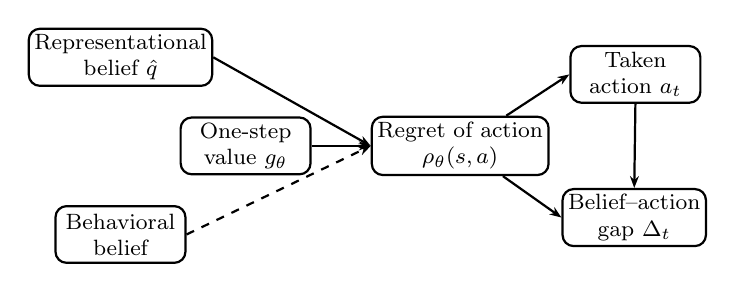
\begin{tikzpicture}[
    node distance=0.45cm and 0.6cm,
    every node/.style={font=\footnotesize,align=center},
    box/.style={rounded corners,draw=black,thick,minimum height=0.72cm,minimum width=1.65cm,inner sep=2pt},
    arrow/.style={-{Stealth[length=1.5mm]},thick}
]
\node[box] (beh) {Behavioral\\belief};
\node[box,above=1.5cm of beh] (rep) {Representational\\belief $\hat{q}$};

\node[box,right=0.75cm of $(rep)!0.5!(beh)$] (cost) {One-step\\value $g_\theta$};
\node[box,right=0.75cm of cost] (value) {Regret of action\\ $\rho_\theta(s,a)$};
\node[box,above right=0.15cm and 0.25cm of value] (act) {Taken\\action $a_t$};
\node[box,below right=0.15cm and 0.15cm of value] (gap) {Belief--action\\gap $\Delta_t$};

\draw[arrow] (rep.east) -- (value.west);
\draw[arrow, dashed] (beh.east) -- (value.west);
\draw[arrow] (cost) -- (value);
\draw[arrow] (value) -- (act.west);
\draw[arrow] (value) -- (gap.west);
\draw[arrow] (act.south) -- (gap.north);
\end{tikzpicture}
\caption{Operational decomposition of the belief--action gap. Belief estimators and the one-step cost model jointly define expected action values; the gap compares the taken action against the best action under those inferred values. Behavioral beliefs are only used for probe validation. }
\label{fig:pipeline}
\end{figure}

% [WHITE-BOX OWNER] Keep the next paragraph to 2 sentences. Confirm the final
% location / has_key / door_open numbers and the decoded A* action number.


\subsection{Decoding Beliefs from Activations}

We first test whether task-relevant state variables are available in the
model's activations before comparing them to actions. In the fixed \textit{DoorKeyEnv}
setting, binary state variables are decoded reliably: pre-reasoning probes
recover both \texttt{has\_key} and \texttt{door\_open} with perfect test
accuracy, while post-reasoning probes remain high but weaker
($0.895$ and $0.886$, respectively). Recovery of location is weaker on held-out states,
but pre-reasoning decoded location remains spatially concentrated:
although test accuracy is $0.348$, $95.5\%$ of predictions fall within
one cell of the true position and $99.0\%$ within two cells. Post-reasoning
decoded location is more diffuse ($60.8\%$ within one cell,
$83.5\%$ within two cells).

These results show that the activations contain substantial information about
the agent's current state, especially before reasoning. We therefore use the
representational probes as the formal state-belief for the
belief--action gap computation.

\subsection{Decoding Optimal Actions from Activations}

We next ask whether the same representations support an action-value
structure. We train one-step IRL models that assign scalar values
$g_\theta(s)$ to states and induce action preferences by comparing exact
next states $T(s,a)$ \cite{ng2000algorithms, ziebartMaximumEntropyInverse2008a}. When supervised with the agent's own actions, this
readout is only moderately predictive, with validation accuracy of $0.59$ for both pre- and post-reasoning representations. In contrast, when
the same objective is supervised with optimal actions, recovery is almost perfect, with validation
accuracy above $0.995$.

This asymmetry suggests that the activations contain a coherent signal of
task-optimal geometry that is stronger than that of the agent's actual behaviour. In other words, the representation is more predictive of
what the agent should do than of what it actually does.
A four-room label-control reproduces the same asymmetry under identical
activations and training with only the target label changed
(Appendix Table~\ref{tab:fourroom_appendix}).



%\subsection{State beliefs are available before action}
%Pre-reasoning activations encode task-relevant state information with high accuracy. On the fixed DoorKey setup, linear probes recover the agent's location at $92.8\%$ before reasoning, \texttt{has\_key} at $100\%$, and \texttt{door\_open} at $100\%$; all three degrade after reasoning, especially location ($42.9\%$ post-reasoning). Even when held-out top-1 location accuracy is modest, the pre-reasoning location belief remains spatially concentrated, with $95.5\%$ of test predictions within one cell of the true location and $99.0\%$ within two cells. The same activation features decode A$^*$-optimal actions much better than the agent acts optimally, with a 39--67 point gap between decodable optimality and enacted optimality across the fixed-grid, four-room, and Seed12 evaluations. One-step IRL shows the same asymmetry: optimal-action supervision is recovered near-perfectly, whereas agent-action supervision remains much weaker, which indicates that the representation supports a coherent value ordering more strongly than it reproduces the model's own actions.


% [All authors] Restore a PRE/POST belief visualization here only if an exported
% figure under `figs/` is available and it displaces no stronger result.

\subsection{Reasoning Changes the Gap \& the Belief State}

We compute the belief--action gap at each step using the probe-estimated
belief distribution, the learned next-state value function, and the action
taken at that step (with and without reasoning). Across all 3,194 evaluated
steps, the mean gap decreases from $0.955$ before reasoning to $0.583$ after
reasoning, while mean belief entropy increases from $1.494$ to $2.085$. The
same qualitative pattern holds on the all-probes-correct subset and on the
held-out probe test set; the exact subset values are reported in 
Table~\ref{tab:gap_entropy}.

\begin{table}[t]
\centering
\small
\setlength{\tabcolsep}{4pt}
\begin{tabular}{lrrrrr}
\toprule
\textbf{Subset} & \textbf{$n$} &
\textbf{$\Delta_{\mathrm{pre}}$}&
\textbf{$\Delta_{\mathrm{post}}$}&
\textbf{$H_{\mathrm{pre}}$} &
\textbf{$H_{\mathrm{post}}$} \\
\midrule
All steps & 3194 & 0.955 & 0.583 & 1.494 & 2.085 \\
All probes correct & 2465 & 0.908 & 0.558  & 1.106 & 1.811 \\
Probe test set & 762 & 1.106 & 0.665  & 2.788 & 3.020 \\
\bottomrule
\end{tabular}
\caption{Mean belief--action gap and belief entropy before and after reasoning.}\label{tab:gap_entropy}
\end{table}

The descriptive pattern is that post-reasoning activations become less spatially
precise while the taken action becomes better aligned with the learned
value structure. This supports the interpretation that reasoning changes how
state information is converted into action, rather than merely adding more
accurate information \cite{lanham2023measuring, dong2025emergent}.
Appendix Fig.~\ref{fig:belief_viz_app} shows the same aggregate pattern in a single
trajectory step: the post-reasoning belief is more diffuse, but the taken
action is better aligned with the learned value structure.


\subsection{Correct Reports, Inconsistent Actions}

\begin{figure}[htbp]
\centering
% [All authors] Preserve this wall-gap figure in the main body unless a stronger
% causal figure becomes available and page pressure forces a replacement.
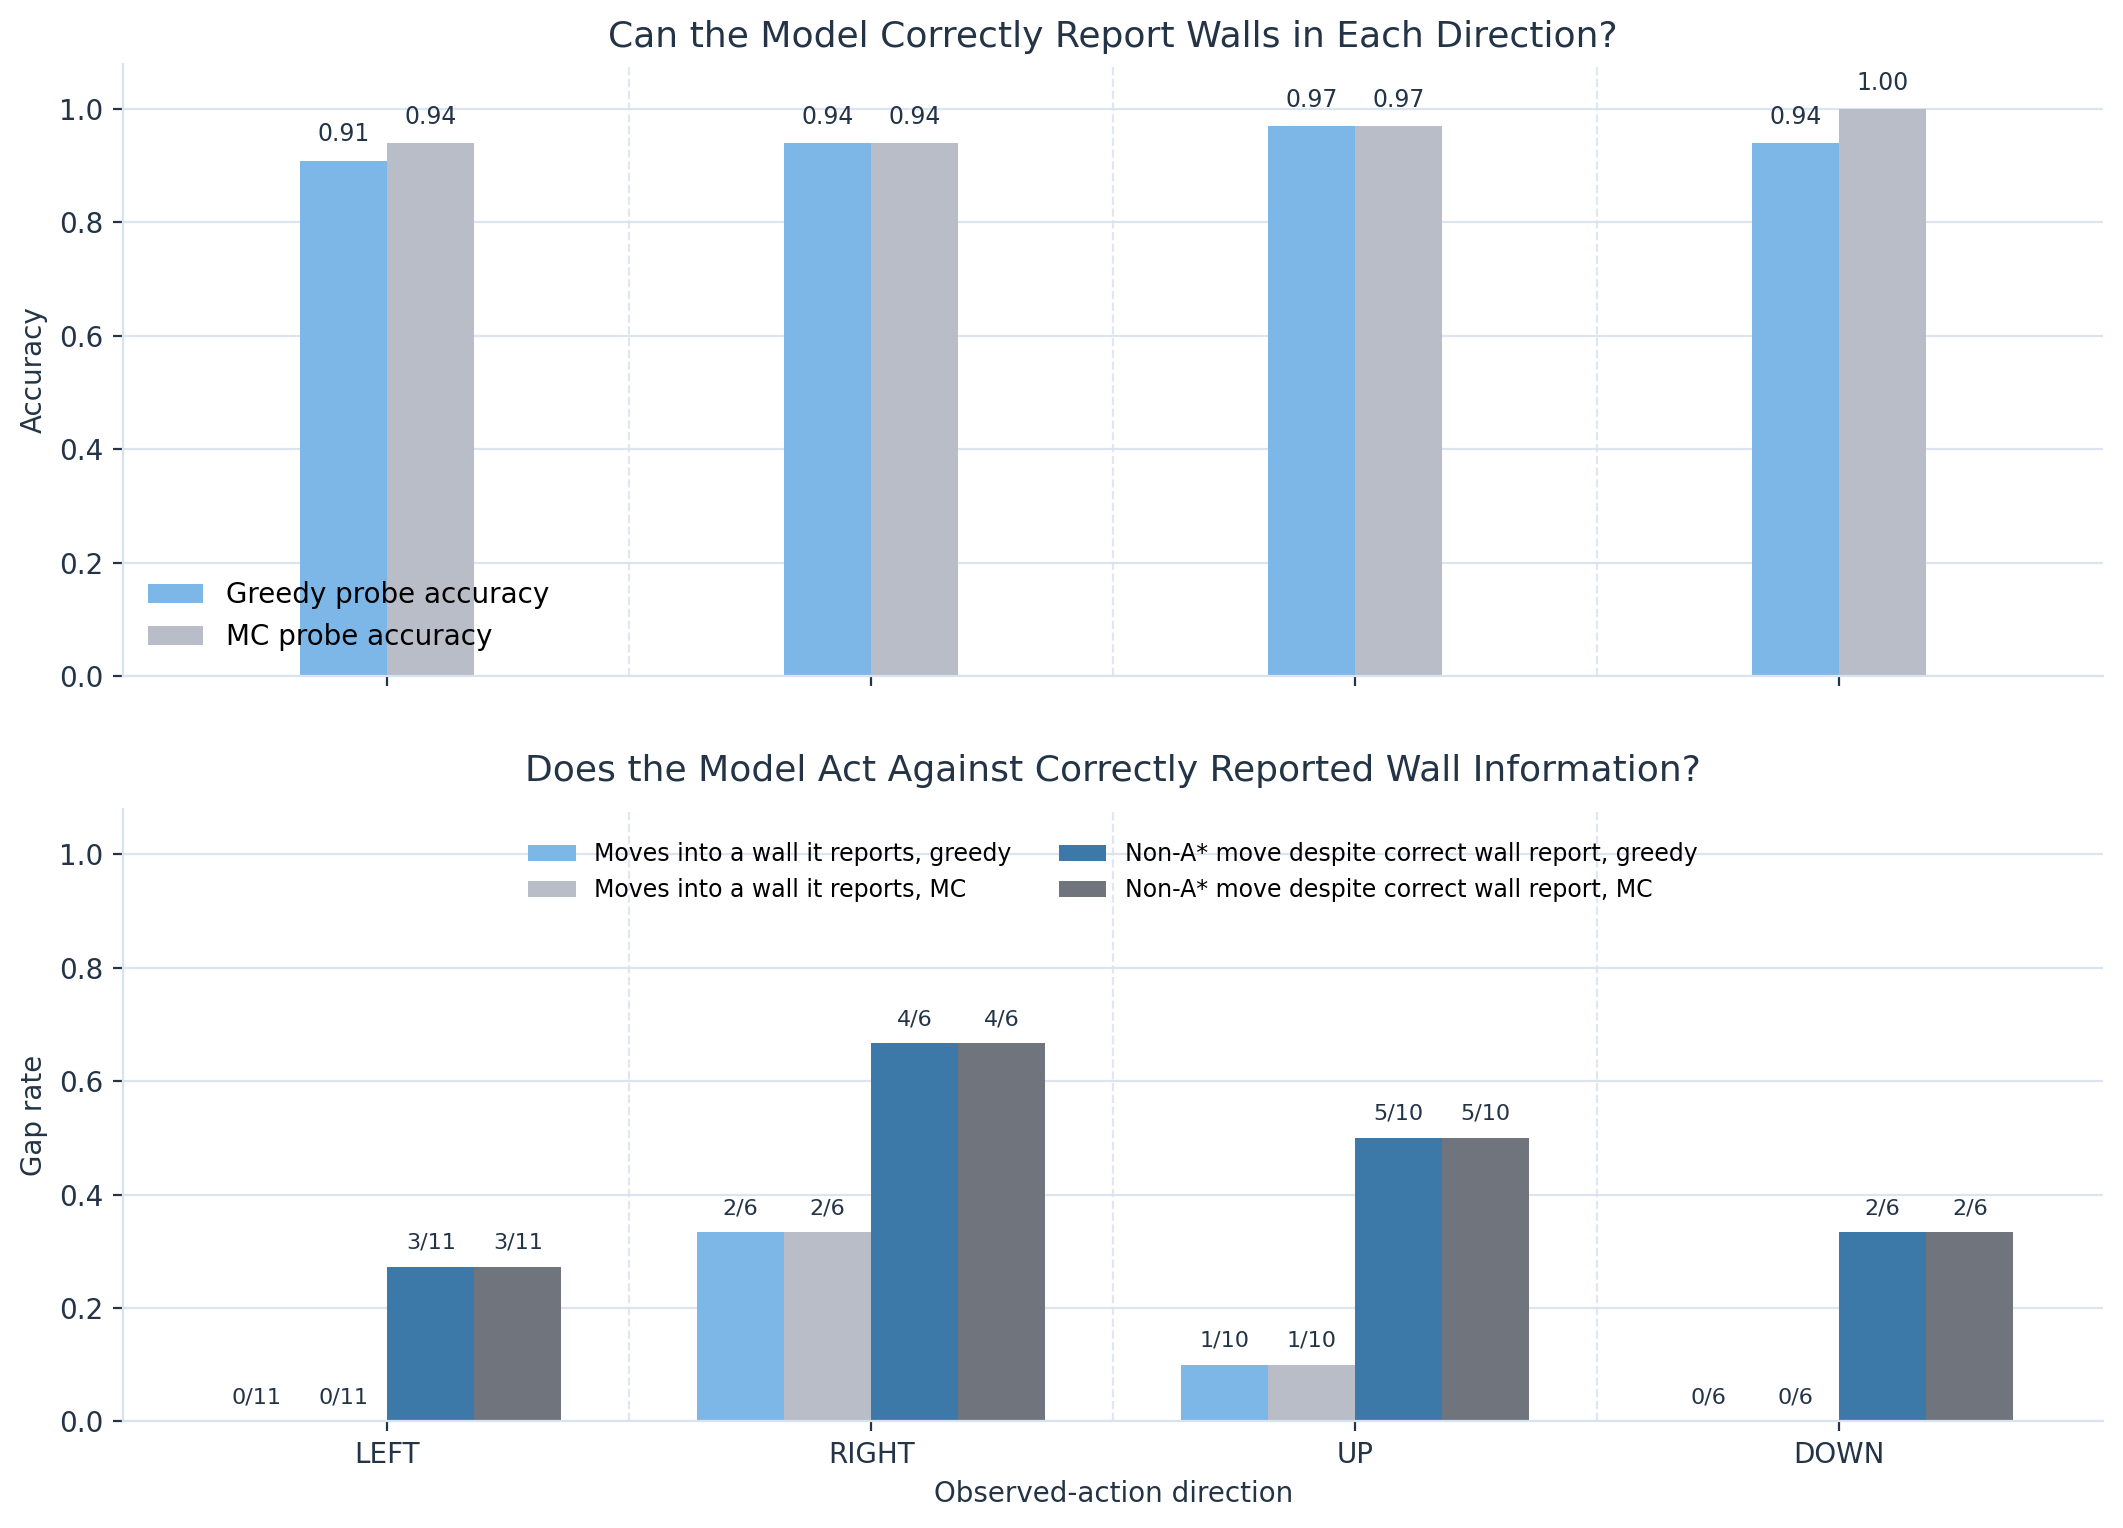
\includegraphics[width=\linewidth]{figs/belief_action_gap_summary_wall_gap.png}
\caption{Wall-probe accuracy and local mismatch on the failure-focused wall slice.}
\label{fig:wall_gap_main}
\end{figure}




As a complementary black-box diagnostic, we also query the model directly
about local state facts. Directional wall probes ask whether the cell adjacent to the agent in a given direction is blocked \cite{arghal2026behavioural, martorell_text_2026}. These
queries test whether relevant local facts are explicitly
recoverable from the model at failure states.

On the expanded wall-focused failure slice, directional wall accuracy remains
high across directions, but action-facing contradiction metrics are non-zero.
The clearest case occurs for wall hits: in all $3/3$ eligible wall-hit cases,
the model correctly reports that the chosen direction is blocked and
nevertheless emits that blocked move. Avoidable detours also show substantial
A$^\ast$-conditioned mismatch despite correct wall judgments. 
Fig.~\ref{fig:wall_gap_main} summarizes the wall-specific result. Accurate wall reports do not guarantee action consistency. This pattern is better classified as an action-selection failure than as a belief failure, because the relevant local fact is behaviorally recoverable at the same state \cite{greenblatt2024faking, vanderweij2025sandbagging}.
Broader behavioral-probe accuracy patterns and selected wall-hit cases are
reported in Appendix Figs~\ref{fig:behavioral_probe_overview_appendix}
and~\ref{fig:wall_hit_cases_appendix}.

\subsection{Behavioral--Representational Agreement on Matched Clean States}

The behavioral estimator is validated on a matched public clean slice of 15
size-7 states drawn from released GPT-OSS-20B trajectories with paired
pre-/post-reasoning activations and cognitive probes \cite{openai2025gptoss120bgptoss20bmodel}. Table~\ref{tab:agreement}
shows that black-box wall readouts are perfect at both $0\%$ and $100\%$
revealed chain-of-thought, while white-box wall decoding is strong but
direction-dependent. This is a validation result on exact matched states, not a
failure-focused slice.

\begin{table}[t]
\centering
\scriptsize
\setlength{\tabcolsep}{3.5pt}
\begin{tabular}{@{}lcccccc@{}}
\toprule
\textbf{Wall} &
\textbf{WB pre} &
\textbf{BB 0\%} &
\textbf{Agr.} &
\textbf{WB post} &
\textbf{BB 100\%} &
\textbf{Agr.} \\
\midrule
\texttt{down}  & 0.800 & 1.000 & 0.800 & 0.933 & 1.000 & 0.933 \\
\texttt{left}  & 0.733 & 1.000 & 0.733 & 0.733 & 1.000 & 0.733 \\
\texttt{right} & 0.867 & 1.000 & 0.867 & 0.933 & 1.000 & 0.933 \\
\texttt{up}    & 1.000 & 1.000 & 1.000 & 0.933 & 1.000 & 0.933 \\
\bottomrule
\end{tabular}
\caption{Matched clean public slice ($N=15$ per wall question). WB = white-box representational probe; BB = black-box behavioral probe. For the black-box probe, $0\%$ and $100\%$ denote no prior chain-of-thought versus full prior chain-of-thought revealed in the behavioral prompt.}\label{tab:agreement}
\end{table}


%\subsection{Additional Label-Control Evidence}

%A four-room label-control experiment gives the same qualitative picture in a separate setting. Holding the activations, architecture, and training procedure fixed, the readout predicts full-state BFS-optimal actions with $96.0\%$ test accuracy and $99.2\%$ optimal-set membership. The same setup predicts the agent's own actions with only $45.4\%$ accuracy, below the majority-class baseline. This strengthens the conclusion that the representations encode task geometry more reliably than they encode the agent's behavioural action bias. 
%Together, these descriptive results motivate the causal analyses that follow: state and value information are recoverable from the model, but the emitted action does not always reflect that information.




%\subsection{Reasoning changes the gap and the belief state}
%Reasoning changes both action-value alignment and state uncertainty. Across all 3,194 evaluated steps, the mean inferred belief--action gap decreases from $0.955$ before reasoning to $0.583$ after reasoning, while mean belief entropy increases from $1.494$ to $2.085$; both changes are significant at $p<0.0001$. The same qualitative pattern holds on the all-probes-correct subset and on held-out probe-test states. At the descriptive level, reasoning improves action-value alignment while making the inferred state representation more diffuse.

% [Behavioral owner] Keep Section 4 focused on the action-selection-failure claim.
% If page pressure is high, preserve the main failure-state figure before adding
% additional descriptive diagnostics.
%\subsection{Failure-focused wall-gap evidence}
%Behavioral probes on failure states provide direct evidence for action-selection failure. On the expanded wall-focused slice of 33 tagged failure states, directional wall accuracy remains high across directions, yet the action-facing contradiction metrics are non-zero. In particular, the model correctly reports that the chosen direction is blocked and still takes that move in all $3/3$ eligible wall-hit cases. Avoidable detours also show a substantial A$^*$-conditioned mismatch despite correct wall judgments.



%\subsection{Behavioral--representational agreement on matched clean states}
%The behavioral estimator is validated on a public matched clean slice of 15 size-7 state snapshots from four released GPT-OSS-20B trajectories, paired with released pre- and post-reasoning activations and cognitive probes. Behavioral wall probes are run on the same $(\text{trajectory},\text{step})$ states. Table~\ref{tab:agreement} shows that black-box wall readouts are perfect at both $0\%$ and $100\%$ revealed chain-of-thought, while white-box wall decoding is strong but direction-dependent. This slice validates the behavioral estimator; it is not a failure-diagnostic slice.

%\begin{table}[htbp]
%\centering
%\scriptsize
%\setlength{\tabcolsep}{3.5pt}
%\caption{Behavioral--representational agreement on matched public size-7 wall states ($N=15$ for all rows). WB = white-box; BB = black-box; Agr. = white-box/black-box agreement.}
%\label{tab:agreement}
%\begin{tabular}{@{}lcccccc@{}}
%\toprule
%\textbf{Wall} &
%\textbf{WB pre} &
%\textbf{BB 0\%} &
%\textbf{Agr.} &
%\textbf{WB post} &
%\textbf{BB 100\%} &
%\textbf{Agr.} \\
%\midrule
%\texttt{down}  & 0.800 & 1.000 & 0.800 & 0.933 & 1.000 & 0.933 \\
%\texttt{left}  & 0.733 & 1.000 & 0.733 & 0.733 & 1.000 & 0.733 \\
%\texttt{right} & 0.867 & 1.000 & 0.867 & 0.933 & 1.000 & 0.933 \\
%\texttt{up}    & 1.000 & 1.000 & 1.000 & 0.933 & 1.000 & 0.933 \\
%\bottomrule
%\end{tabular}
%\end{table}
% [All authors] If page pressure becomes severe after adding the causal result,
% Table 1 is the first descriptive item that can move to the appendix.

%\subsection{Additional descriptive diagnostics}
%The four-room label-control result strengthens the action-selection interpretation. Holding activations, architecture, and training procedure fixed, the same features predict full-state BFS-optimal actions at $96.0\%$ accuracy and $99.2\%$ optimal-set membership, but predict the agent's own actions only $45.4\%$, below the majority baseline. This shows that the representation is much more predictive of optimal geometry than of the agent's behavioral action bias.

\section{Causal Tests on Reasoning Trajectories}
To evaluate whether the belief--action gap is causally implicated in the model's final decisions, we intervene on trajectory representations around the reasoning trace \cite{meng2022locating, kramar2024atpstar}.

\subsection{Intervention setup}
We use two complementary intervention families. First, we patch reasoning
trajectories by combining the input state from one sample with the reasoning
trace from another, testing whether the final action follows the original
state or the transplanted reasoning. Second, we steer or swap activation
representations at selected layers and token positions, including
pre-reasoning suffix positions and final action-adjacent positions. These
interventions test whether decodable state or action variables are merely
available to probes, or actually lie on the pathway used to produce the final
action.

%\subsection{Patching and steering results}
%Reasoning-trace interventions indicate that the final action is controlled bythe reasoning trace rather than by the pre-reasoning state representation alone. In the patching experiment $f(X_1, R_2)=Y_{12}$, the patched trajectories satisfy $Y_{12}=Y_2$ in $100\%$ of cases, with a $76\%$ flip raterelative to the baseline action. By contrast, interventions on pre-reasoning activations alone have no detectable effect. This supports a routing account:task-relevant information is present before reasoning, but the reasoning trace redirects the computation toward a later action commitment. The steering results sharpen this account: in the corrected verbose-prompt flag-swap experiment, causal control appears only when the intervention matches the relevant layer, prompt format, and baseline action direction, 



\subsection{Patching and steering results}

Reasoning-trace patching indicates that the final action is strongly
controlled by the reasoning trajectory. With input $X$, reasoning $R$, output $Y$ and the LM $f$, we want to establish the causal effect of $X$ and $R$ to $Y$. Assuming two samples $(X_1, R_1, Y_1)$ and $(X_2, R_2, Y_2)$, and doing inference with
$f(X_1,R_2)=Y_{12}$, the patched output follows the donor reasoning action:
$Y_{12}=Y_2$ in $100\%$ of tested cases, with a $76\%$ flip rate relative to
the original baseline action. This suggests that once a reasoning trajectory
is fixed, the final action is routed through that trajectory rather than
through the original input state alone.

By contrast, simple interventions on pre-reasoning activations provide little
evidence of direct causal control. Swapping pre-reasoning activations between
different starting states, and steering pre-reasoning activations before
regenerating the chain of thought, did not reliably change the final output.
Thus, pre-reasoning activations can encode task-relevant information without
being a sufficient causal bottleneck for action generation, which indicates
that the relevant representation must lie on the action-generation pathway used
by that prompt \cite{kramar2024atpstar}. Appendix Table~\ref{tab:causal_summary_appendix} summarizes the
intervention results.

\subsection{Steering Depends on Layer and Position}

The steering results show that interventions do not work uniformly across
settings. Changing a representation affects the final action only when the
intervention is applied at the right layer and token position, and when the
steering direction matches the action the model would otherwise take. In the
corrected verbose-prompt swaps, changing pre-reasoning or suffix-level belief
representations was not enough to redirect the action. By contrast, steering
near the action output can change the model's choice when the intervention is
defined relative to the model's actual baseline action. Appendix ~\ref{app:probe_steering} describes the process in more detail. 



\begin{table}[t]
\centering
\scriptsize
\setlength{\tabcolsep}{3.5pt}
\begin{tabular}{rccccc}
\toprule
\textbf{Reveal (\%)} & \textbf{Wall acc.} & \textbf{Wall ent.} & \textbf{MC act. ent.} & \textbf{Local gap} & \textbf{$A^\ast$ gap} \\
\midrule
0   & 0.942 & 0.000 & 0.283 & 0.000 & 0.000 \\
25  & 0.942 & 0.000 & 0.141 & 0.077 & 0.083 \\
50  & 0.962 & 0.000 & 0.141 & 0.154 & 0.231 \\
75  & 0.942 & 0.000 & 0.141 & 0.077 & 0.385 \\
100 & 0.942 & 0.000 & 0.000 & 0.231 & 0.538 \\
\bottomrule
\end{tabular}
\caption{Focused failure-slice behavioral results by revealed reasoning level.}\label{tab:focused_failure_slice}
\end{table}


\subsection{Auxiliary revealed-CoT diagnostic}
The reasoning-trajectory analysis uses a behavioral-only failure slice: 4 avoidable-detour steps, 3 wall-hit steps, 2 backtracks, and 4 optimal baseline steps from local GPT-OSS-20B chain-of-thought trajectories. Revealed reasoning is varied at $0,25,50,75,100\%$ of the released analysis text, while the original final JSON action is never shown.

Internal pre/post analyses motivate this experiment: after reasoning, the inferred gap is lower while state uncertainty is higher. The behavioral revealed-CoT result does not show the same pattern: wall-belief accuracy and wall entropy remain effectively flat, while Monte Carlo-sampled action entropy decreases and both local and A$^\ast$-conditioned gap rates rise. Table~\ref{tab:focused_failure_slice} reports the reveal-level values for this focused failure slice. Revealed reasoning text is therefore not a reliable external proxy for improved behavioral belief--action alignment \cite{lanham2023measuring, li2025spilling, marks2025auditing}.



\section{Discussion}
The results support that some agent failures are not due to state representation. Task-relevant information is available both representationally and behaviorally, yet the taken action can still be inconsistent with that information. Pre-reasoning activations encode optimal-action structure much more strongly than the model acts on it, reasoning reduces the inferred gap while increasing belief uncertainty, and wall-hit failures show that explicit local knowledge can still coexist with inconsistent action. The clean matched slice shows that representational and behavioral wall probes target similar state information.

The main causal result is not the auxiliary revealed-CoT diagnostic but the intervention evidence on reasoning traces. Patching shows that the reasoning trace, rather than the pre-reasoning state representation alone, determines the final action, and steering shows that this causal control is specific to the relevant layer, prompt format, and action direction. The revealed-CoT analysis remains useful as a behavioral-only negative control: exposing more prior reasoning text does not repair the behavioral gap. 






\section{Conclusion}
This work introduces the belief--action gap as a framework for separating failures of state representation from failures of action selection in LM agents. Across text-rendered grid environments, task-relevant state information and objective-consistent value structure are often recoverable from both internal representations and behavioral probes even when the taken action is suboptimal. Representations therefore encode optimal-action structure more reliably than the model’s realized behavior, and explicit local knowledge can coexist with inconsistent actions.


Causal interventions further indicate that final actions depend more strongly on later reasoning representations than on pre-reasoning state information alone. Together, these findings support a view of LM-agent failures in which relevant knowledge is available but not consistently translated into behavior. The belief--action gap therefore provides a useful diagnostic lens for studying when agents know, reason about, and ultimately fail to act on task-relevant information.





%\bibliographystyle{plain}
\bibliography{refs}


\appendix

%\section{Appendix Summary}
%This appendix collects supporting results referenced in the main text. Appendix Section~\ref{app:environment} summarizes the DoorKey task setup used in
%Section 2, Appendix Table~\ref{tab:causal_summary_appendix} expands the causal intervention summary from Section 4, Appendix Table~\ref{tab:fourroom_appendix} supports the action-decoding asymmetry described in Section 2, and Appendix Figures~\ref{fig:behavioral_probe_overview_appendix} and~\ref{fig:wall_hit_cases_appendix} provide broader behavioral evidence for the failure-state discussion in Section 3.


\section{Limitations}
These results come from controlled grid
environments with deterministic transitions and fully observ-
able states. The one-step IRL estimator is an operational ap-
proximation to action value rather than a full long-horizon
model of planning, the probes estimate internal state rather than
measuring exact belief directly, and the intervention results are
established only for the evaluated model family and prompt
conditions.

\section{\textit{DoorKeyEnv} Summary}
\label{app:environment}
The experiments use text-rendered gridworlds, \textit{DoorKeyEnv}, with deterministic
transitions and fully observed layouts. At each step the agent receives the
current grid rendering and must choose one of the cardinal moves; the task is
to reach the goal cell while respecting walls and, in key-door variants,
retrieving a key before opening a locked door. The state variables used in the
belief estimators are the agent's grid location $(x_t,y_t)$ together with the
binary task variables \texttt{has\_key} and \texttt{door\_open}. The one-step
IRL model evaluates each candidate move by applying the exact transition
function $T(s_t,a)$ to the current state and comparing the values of the
resulting next states.
\begin{figure}[!ht]
\centering
    \centering
    \begin{BVerbatim}
  0 1 2 3 4 5 6 
0 # # # # # # # 
1 # A . . # G # 
2 # . # _ # . # 
3 # . K _ D . # 
4 # . . . # . # 
5 # . . . # # # 
6 # # # # # # # 
    \end{BVerbatim}
%\fbox{%
%\begin{minipage}{0.55\columnwidth}
%\small
%\centering
%\ttfamily
%\begin{tabular}{ccccccc}
%\# & \# & \# & \# & \# & \# & \# \\
%\# & A  & .  & .  & \# & G  & \# \\
%\# & .  & \# & .  & \# & .  & \# \\
%\# & .  & K  & .  & D  & .  & \# \\
%\# & .  & .  & .  & \# & .  & \# \\
%\# & \# & \# & \# & \# & \# & \#
%\end{tabular}
%\end{minipage}}
\caption{Example text-rendered \textit{DoorKeyEnv}. `A` is the agent, `G` the goal,
`K` the key, `D` the door, `#` walls, and `.` free cells. Some environments
omit the key-door dependency; in those cases the agent only needs to navigate
to the goal while avoiding walls.}
\label{fig:doorkey_example_appendix}
\end{figure}

\section{Additional Experimental Results}

\subsection{Causal Intervention Summary}
\label{app:causal_summary}
This table gives the quantitative summary behind the causal claims in
Section 4. 

\begin{table}[htbp]
\centering
\scriptsize

\begin{tabularx}{\columnwidth}{@{}p{0.29\columnwidth}p{0.28\columnwidth}X@{}}
\toprule
\textbf{Intervention} & \textbf{Observed result} & \textbf{Interpretation} \\
\midrule
Reasoning-trace patching $f(X_1, R_2)=Y_{12}$ & $Y_{12}=Y_2$ in $100\%$ of cases; $76\%$ flip rate & Final action follows the patched reasoning trace rather than the original pre-reasoning state representation. \\
Pre-reasoning activation patching only & No detectable effect & Correct pre-reasoning information is not, by itself, sufficient to determine the final action. \\
Verbose-prompt flag-swap steering & Control only when layer, prompt format, and baseline direction match & Causal control is pathway-specific rather than a generic readout of the suffix representation. \\
\bottomrule
\end{tabularx}
\caption{Summary of causal interventions on reasoning trajectories.}\label{tab:causal_summary_appendix}
\end{table}

\subsection{Four-Room Label-Control Result}
\label{app:fourroom}
The four-room control keeps the activations, architecture, and training procedure fixed while changing only the target label. Table~\ref{tab:fourroom_appendix} shows that the same representation predicts full-state BFS-optimal actions much better than the agent's own actions.

\begin{table}[!ht]
\centering
\small
\begin{tabular}{lrr}
\toprule
\textbf{Metric} & \textbf{Agent action} & \textbf{BFS-optimal} \\
\midrule
Test accuracy & 0.454 & 0.960 \\
Test set-membership accuracy & 0.369 & 0.992 \\
Test log-likelihood & $-0.9969$ & $-0.1389$ \\
Train accuracy & 0.451 & 0.972 \\
Majority-class baseline & 0.548 & 0.733 \\
Random baseline & 0.250 & 0.250 \\
\bottomrule
\end{tabular}
\caption{Four-room label-control result. Identical activations and algorithm; only the label changes.}
\label{tab:fourroom_appendix}
\end{table}

\subsection{Additional Behavioural Evidence}
\label{app:behavioral_more}
These figures provide broader support for the behavioral interpretation in
Section 3. Fig.~\ref{fig:behavioral_probe_overview_appendix} summarizes the
accuracy pattern across question families, and
Fig.~\ref{fig:wall_hit_cases_appendix} shows concrete wall-hit and
sub-optimality examples behind the aggregate contradiction metrics.

\begin{figure*}[!ht]
\centering
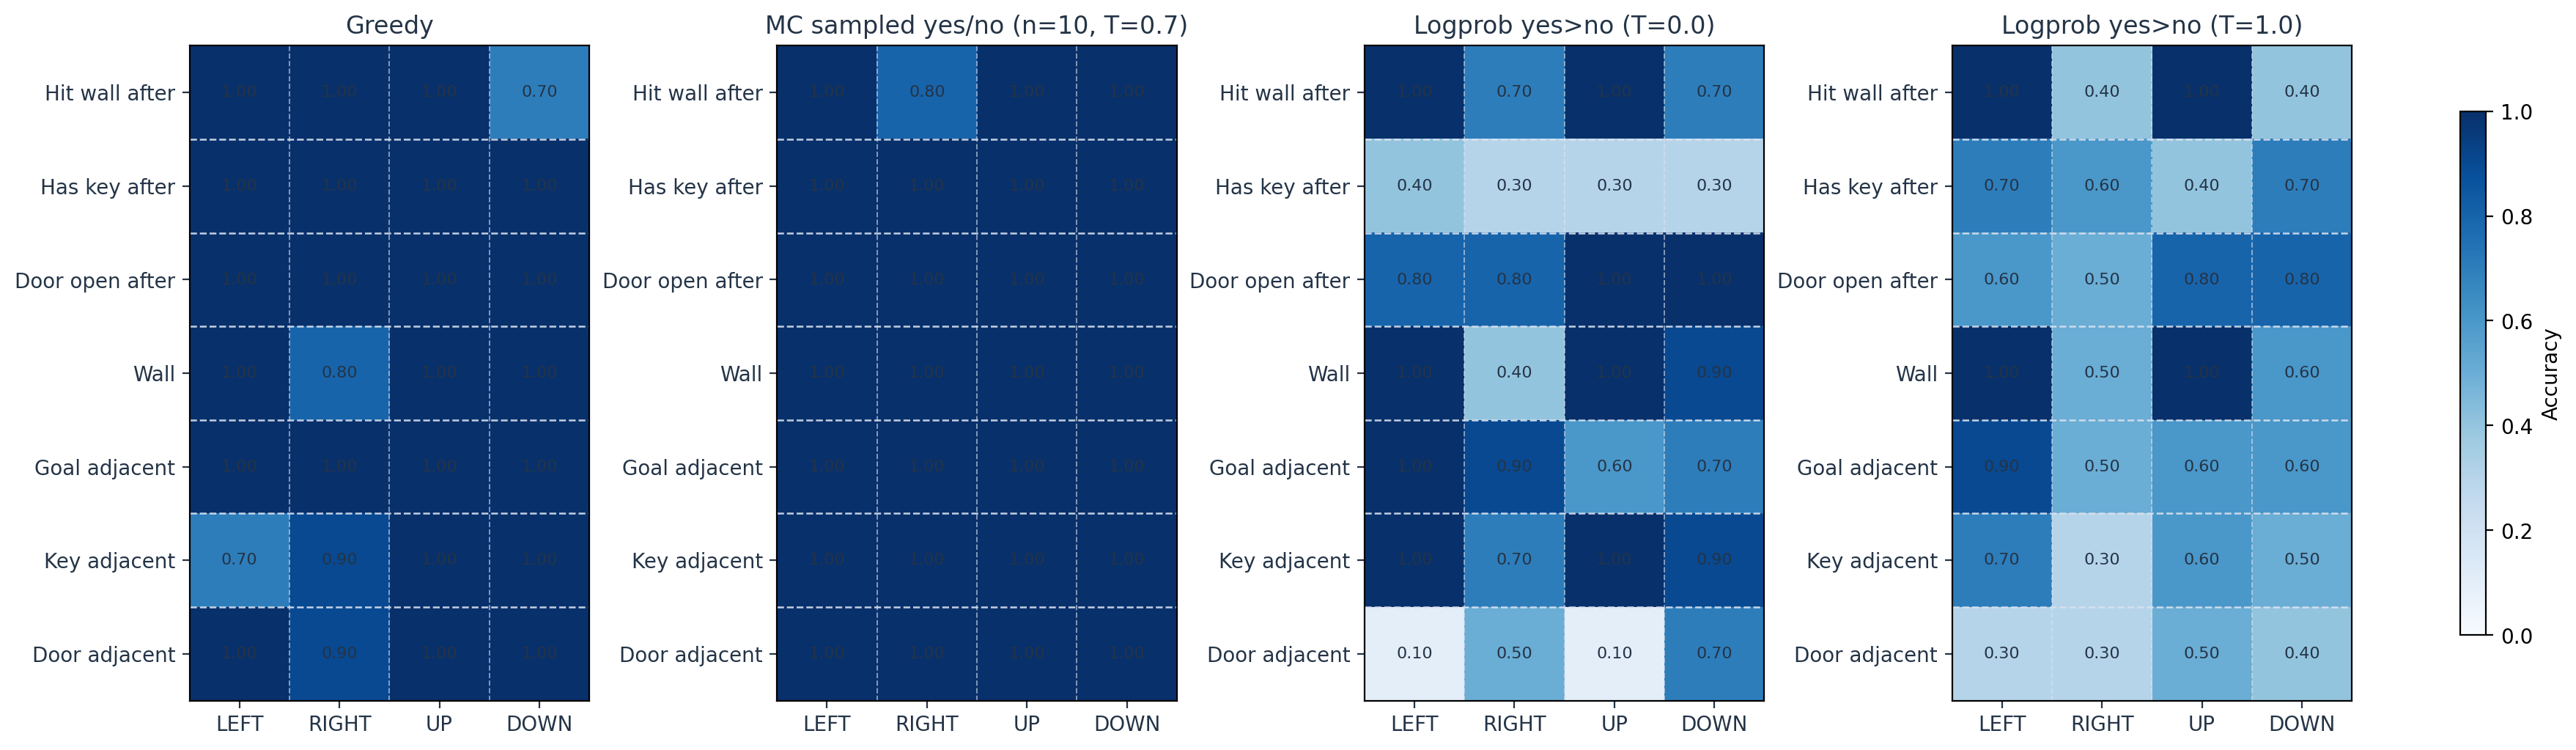
\includegraphics[width=\linewidth]{figs/behavioral_probe_directional_heatmap_overview.png}
\caption{Broader behavioural-probe accuracy across directional question families. Wall, goal, and door probes are generally strong, whereas key-direction judgements are less reliable.}
\label{fig:behavioral_probe_overview_appendix}
\end{figure*}

\begin{figure}[!ht]
\centering
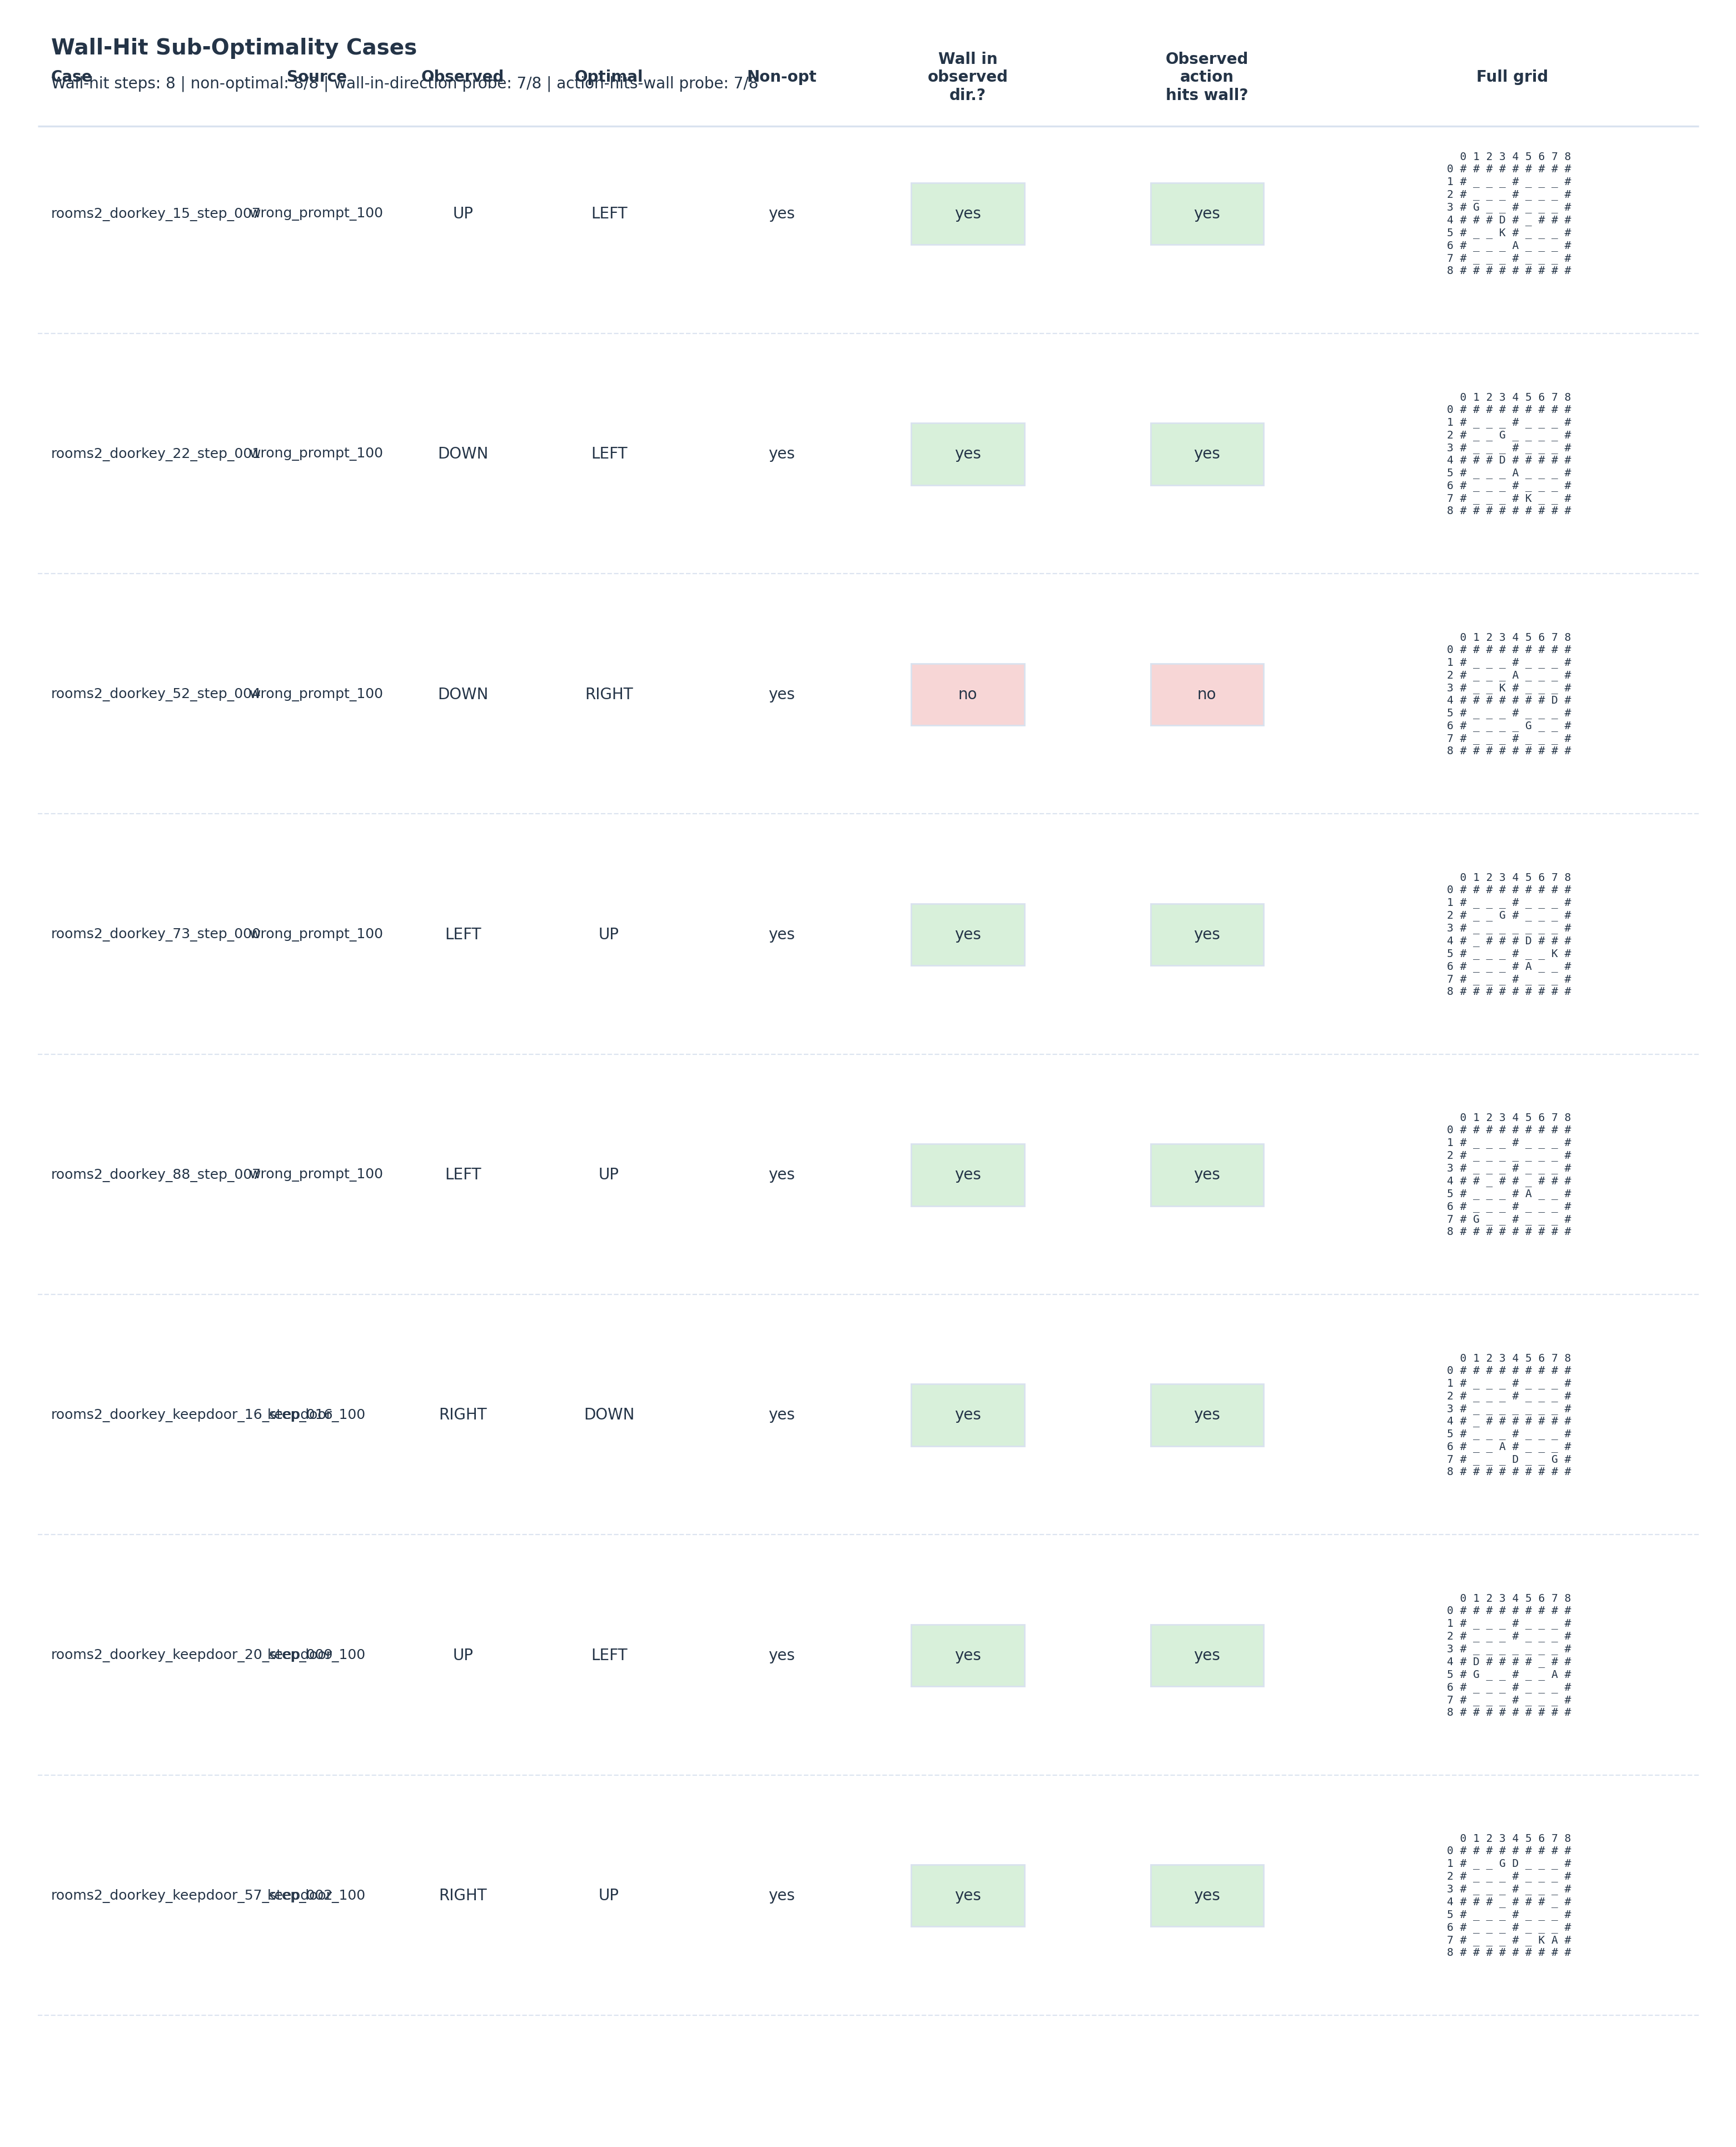
\includegraphics[width=\linewidth]{figs/wall_hit_suboptimality_cases.png}
\caption{Selected wall-hit and sub-optimality cases in which the model reports the local wall fact correctly yet still takes a wall-hitting or non-optimal action.}
\label{fig:wall_hit_cases_appendix}
\end{figure}


\section{Additional Descriptive Results for Belief--Action Gap Estimation}
\label{app:descriptive_results}

This appendix reports additional probe, IRL, and GAP diagnostics supporting the
descriptive results in the main text.

\subsection{Probe Results}
\label{app:probe_results}

We evaluate the six trained state probes using top-1 accuracy and, for the
location probe, spatial concentration around the true position. The latter is
important because the GAP computation uses the full belief distribution
$q_t$, not only the top-1 prediction.

\paragraph{Binary probes.}
The \texttt{has\_key} and \texttt{door\_open} probes achieve near-perfect
accuracy (Table~\ref{tab:binary_probe_acc_app}). PRE probes are perfect on the
test set, while POST probes remain high but weaker.

\begin{table}[!ht]
\centering
\small
\begin{tabular}{llcc}
\toprule
\textbf{Probe} & \textbf{Position} & \textbf{Train Acc.} & \textbf{Test Acc.} \\
\midrule
$\hat{q}^{\textit{hk}}$  & PRE  & 1.000 & 1.000 \\
$\hat{q}^{\textit{hk}}$  & POST & 1.000 & 0.895 \\
$\hat{q}^{\textit{do}}$  & PRE  & 1.000 & 1.000 \\
$\hat{q}^{\textit{do}}$  & POST & 1.000 & 0.886 \\
\bottomrule
\end{tabular}
\caption{Train and test accuracy for binary state probes.}
\label{tab:binary_probe_acc_app}
\end{table}

\paragraph{Location probe.}
Location top-1 accuracy is modest on held-out states, especially after
reasoning, but the predicted locations remain spatially concentrated around the
true position (Table~\ref{tab:loc_probe_acc_app}). For PRE activations,
$95.5\%$ of test predictions fall within one cell of the true position and
$99.0\%$ within two cells. POST activations are less precise, with $60.8\%$
within one cell and $83.5\%$ within two cells.

\begin{table}[!ht]
\centering
\small
\begin{tabular}{lccccc}
\toprule
\textbf{Position} & \textbf{Split} & \textbf{Acc.} & \textbf{L1 mean}  & $\leq 1$ & $\leq 2$ \\
\midrule
PRE  & Train & 1.000 & 0.000 & 100.0\% & 100.0\% \\
PRE  & Test  & 0.348 & 0.717 &  95.5\% &  99.0\% \\
POST & Train & 1.000 & 0.001 & 100.0\% & 100.0\% \\
POST & Test  & 0.131 & 1.585 &  60.8\% &  83.5\% \\
\bottomrule
\end{tabular}
\caption{Location probe accuracy and distance metrics. $\leq d$ denotes the
percentage of predictions within L1 distance $d$ of the true position.}
\label{tab:loc_probe_acc_app}
\end{table}

\paragraph{Accumulated probability mass.}
Table~\ref{tab:vicinity_prob_app} reports the mean probability mass assigned by
the location probe to all walkable cells within L1 distance $n$ of the true
position. The PRE belief places $93.1\%$ of its mass within one cell and
$97.2\%$ within two cells. POST beliefs are more diffuse but still place most
mass within two cells.

\begin{table}[!ht]
\centering
\small
\begin{tabular}{lcccccc}
\toprule
\textbf{Position} & $n=0$ & $n=1$ & $n=2$ & $n=3$ & $n=4$ & $n=5$ \\
\midrule
PRE  & 0.347 & 0.931 & 0.972 & 0.986 & 0.993 & 0.997 \\
POST & 0.127 & 0.592 & 0.815 & 0.892 & 0.945 & 0.975 \\
\bottomrule
\end{tabular}
\caption{Mean accumulated probability mass within L1 distance $n$ of the true
position on the probe test set.}
\label{tab:vicinity_prob_app}
\end{table}

Overall, POST location readouts are weaker and more diffuse than PRE readouts,
consistent with the main-text finding that reasoning reduces the GAP while
increasing belief uncertainty.

\subsection{IRL Value Function Validation}
\label{app:irl_validation}

To check that the learned $g_\theta$ captures meaningful next-state preferences
rather than simply memorising action labels, we train an additional IRL model
using optimal actions computed by an A* planner. Table~\ref{tab:irl_comparison_app}
compares agent-action and optimal-action supervision.

\begin{table}[!ht]
\centering
\small
\begin{tabular}{llcc}
\toprule
\textbf{Representation} & \textbf{Supervision} & \textbf{Train Acc.} & \textbf{Val Acc.} \\
\midrule
PRE  & Agent action   & 0.598 & 0.588 \\
PRE  & Optimal action & 0.998 & 0.997 \\
POST & Agent action   & 0.607 & 0.590 \\
POST & Optimal action & 0.995 & 0.995 \\
\bottomrule
\end{tabular}
\caption{IRL accuracy under agent-action and optimal-action supervision for PRE
and POST representations.}
\label{tab:irl_comparison_app}
\end{table}

Optimal-action supervision reaches near-perfect validation accuracy
($\geq 99.5\%$), while agent-action supervision remains around $59\%$. This
asymmetry suggests that the activations support a coherent task-value ordering
more strongly than they reproduce the model's own inconsistent action choices.

\begin{figure*}[t]
    \centering
    \includegraphics[width=0.8\textwidth]{figs/traj196_step5_pre_value_compare.pdf}
    \caption{Learned $g_\theta(s)$ values across the grid for
    optimal-action-supervised IRL (left) and agent-action-supervised IRL
    (right), both using POST representations. Darker cells indicate higher
    learned value. Both landscapes show structured value variation around the
    key, door, and goal regions, supporting the interpretation of $g_\theta$ as
    a global next-state preference function rather than a memorized action
    classifier.}
    \label{fig:irl_value_app}
\end{figure*}









\begin{figure*}[]
    \centering
    \includegraphics[width=0.8\textwidth]{figs/traj192_step5.pdf}
    \caption{Example PRE/POST belief--action gap visualization. Cell numbers
    show the probe-estimated location probabilities, with shading proportional
    to probability mass. Arrows mark the next state preferred by the learned
    value function and the action actually taken by the agent. In this
    example, reasoning makes the location belief more diffuse
    ($H: 0.261 \rightarrow 1.572$) while reducing the expected gap
    ($\mathrm{GAP}: 2.386 \rightarrow 0.205$).}
    \label{fig:belief_viz_app}
\end{figure*}

Fig.~\ref{fig:irl_value_app} visualizes the learned value landscapes. Both
supervision signals recover qualitatively structured values, but optimal-action
supervision yields substantially stronger action prediction.

Fig.~\ref{fig:belief_viz_app} shows a representative example. Before
reasoning, the probe belief is sharply concentrated near the true cell but the
taken action has high expected regret. After reasoning, the belief spreads
over more states, yet the taken action is better aligned with the learned
value function. This illustrates the aggregate pattern: reasoning makes the
state representation more diffuse while reducing the measured belief--action
gap.


\section{Probe-Directed Action Steering in a Door-Key Gridworld}
\label{app:probe_steering}

We test whether directions from an optimal-action probe can causally steer a
gridworld agent's final action. The task is a $9{\times}9$ DoorKey gridworld
with four possible actions: \texttt{LEFT}, \texttt{RIGHT}, \texttt{UP}, and
\texttt{DOWN}. The model receives the full rendered grid and must emit a JSON
action. Optimal targets are computed by A* search in the environment, rather
than taken from the model's recorded trajectory action.

\paragraph{Example.}
Symbols follow the usual grid convention: \texttt{\#} is a wall, \texttt{\_} is
open space, \texttt{A} is the agent, \texttt{G} is the goal, and \texttt{K} is
the key. One steering example is shown below.

\begin{verbatim}
  0 1 2 3 4 5 6 7 8
0 # # # # # # # # #
1 # _ _ _ # G _ _ #
2 # _ _ _ # _ _ _ #
3 # _ _ _ _ _ _ _ #
4 # _ # # # # # # #
5 # _ _ A # K _ _ #
6 # _ _ _ # _ _ _ #
7 # _ _ _ _ _ _ _ #
8 # # # # # # # # #

Agent status:
- Carrying key: False
- Door open: True
- A* optimal next action: LEFT
\end{verbatim}

For this state, one no-hook sampled baseline emitted \texttt{RIGHT}, which is
not A*-optimal. Steering from the baseline action \texttt{RIGHT} toward the
A* target \texttt{LEFT} changed the paired completion to \texttt{LEFT}.

\begin{figure*}[t]
    \centering
    \includegraphics[width=\linewidth]{figs/action_probe_direction_steering_summary.png}
    \caption{
    Probe-directed steering from a nonoptimal baseline action toward an
    A*-optimal target. The main comparison is between steering toward an
    A*-optimal action and steering toward wrong actions under the same prompt,
    seed, layer, and token positions.
    }
    \label{fig:probe_direction_steering}
\end{figure*}

\paragraph{Method.}
We train a linear optimal-action probe on frozen activations. The probe input is
the mean activation over the final three pre-reasoning prompt-suffix tokens, so
the intervention adds a vector to exactly those three token positions during
the prompt forward pass. For each prompt and random seed, we first generate a
no-hook baseline and parse its action. If the baseline is missing or already
A*-optimal, we skip the pair. Otherwise, the baseline action becomes the source
action $s$. For each candidate target action $c \neq s$, we construct the
probe-margin direction
\[
    d(c,s) =
    \frac{W_c - W_s}{\|W_c - W_s\|},
\]
where $W_c$ and $W_s$ are activation-space probe weights. We then regenerate
with the same prompt and seed after adding
$\alpha \cdot \mathrm{gap}(c,s) \cdot d(c,s)$ at the selected layer. Candidate
targets in the A* optimal set are treated as desired targets; all other
candidate targets are wrong-action controls. This keeps the prompt, seed,
baseline action, layer, and token positions fixed across the desired and
control interventions.

\paragraph{Results.}
The clearest effect occurs at layer 15 with $\alpha=0.5$, using the model's
actual no-hook baseline action as the source. A*-target steering converts
$27/69$ cases to the desired action, while wrong-action controls convert
$32/138$ cases.

\begin{table}[!ht]
\centering
\small
\begin{tabular}{lccc}
\toprule
\textbf{Condition} & \textbf{A* target} & \textbf{Wrong controls} & \textbf{Adv.} \\
\midrule
Layer 15, $\alpha=0.5$ & $27/69=0.391$ & $32/138=0.232$ & $+0.159$ \\
Layer 23, $\alpha=0.5$ & $0/58=0.000$ & $0/116=0.000$ & $0.000$ \\
Layer 23, $\alpha=-1024$ & $8/33=0.242$ & $9/66=0.136$ & $+0.106$ \\
\bottomrule
\end{tabular}
\caption{Probe-directed steering results. Advantage is the A*-target
conversion rate minus the wrong-action control conversion rate.}
\label{tab:probe_direction_steering}
\end{table}

Other direction definitions were also tested. Target-only directions and
directions starting from the recorded trajectory action do not pass the
A*-target-versus-control test. The cleanest moderate-scale result uses the
action actually emitted by the paired no-hook baseline as the source action.

\paragraph{Interpretation.}
This experiment supports a narrow causal claim. On this balanced set of
gridworld prompt states, adding the raw probe-margin direction from the model's
actual nonoptimal baseline action toward an A*-optimal action increases
A*-optimal action emission more than comparable wrong-action control
directions. The effect is not universal: it is strongest for the layer-15
baseline-action-to-A*-target margin, while layer 23 is inert at $\alpha=0.5$
and only shows a weaker effect under an extreme opposite-sign setting. The
effect is also uneven across target labels: \texttt{LEFT}, \texttt{RIGHT}, and
a small \texttt{UP} slice improve in the largest confirmation, while
\texttt{DOWN} does not.

\end{document}
